%!TEX root = ../main.tex
% !TeX spellcheck = en_GB 


\chapter{Implementation}
The objective of this thesis was to implement and evaluate a  collision avoidance  algorithm for USVs. Several related approaches where analysed before the fuzzy logic approach presented by \textcite{perera2012intelligent}, was chosen to be implemented.
The solution presented in the original paper is implemented in MATLAB, while the solution presented here is implemented in Python. Python was chosen due to the writers previous knowledge of the language as well as the availability of fuzzy logic python libraries. The library used in this implementation is called SciKit-Fuzzy \cite{josh_warner_2017_1002946}.
\section{The fuzzy inference system}
The fuzzy logic framework SciKit-Fuzzy is used to implement the model described in section \ref{section:model}. The framework provides a simple API which enables one to define Antecedents, Consequents, their corresponding FMFs as well as the rules that unite them. First antecedents are initialized as shown in listing \ref{listing:ant}
\begin{listing}[ht]
    \begin{minted}{python}
bear = ctrl.Antecedent(np.arange(0, 360, 1), 'bearing')
\end{minted}
    \caption{Antecedent initialization}
    \label{listing:ant}
\end{listing}
This creates the antecedent \textit{bearing} with a universe spanning from 0 to 360 with steps of 1. FMFs are then added to the antecedent. Listing \ref{listing:fmf} shows the FMF for sector II of the model. It starts at 5\textdegree relative bearing and ends at 85\textdegree, with a 5 \textdegree  fuzziness on both sides.
\begin{listing}[ht]
    \begin{minted}{python}
bear['2'] = fuzz.trapmf(bear.universe, generate_trapetzoid(5, 85, 5))
\end{minted}
    \caption{FMF initialization}
    \label{listing:fmf}
\end{listing}

The other antecedents and consequents are initialized and populated with FMFs in the same manner, according to the model described in section \ref{section:model}.

Rules are defined in order to connect the antecedents with consequents.
A rule consist of an antecedent and a consequent as follows:
\begin{minted}{python}
Rule(antecedent, consequent)
\end{minted}
Where the parameter \textit{antecedent} can be a combination of antecedents using the \textit{\&} and \textit{|} operators.
An example based on \ref{rule:1} in section \ref{section:FIS} can be seen in listing \ref{listing:rule}.
\begin{listing}[ht]{}
    \begin{minted}{python}
Rule(
    'II' &
    'f' &
    '>1' &
    ('Rvd'|'Ra'|'Rb'),
    'starboard','decrease')
            
\end{minted}
    \caption{Rule initialization}
    \label{listing:rule}
\end{listing}

These rules are then passed to the ControlSystem that each vessel utilizes to calculate proper course and speed corrections.
\section{Architecture}
This section will present the high level structure of the implementation with the help of the class diagram seen in figure \ref{fig:class_diagram}. Each class and their interactions will be briefly presented.
\begin{figure}[H]
    \centering
    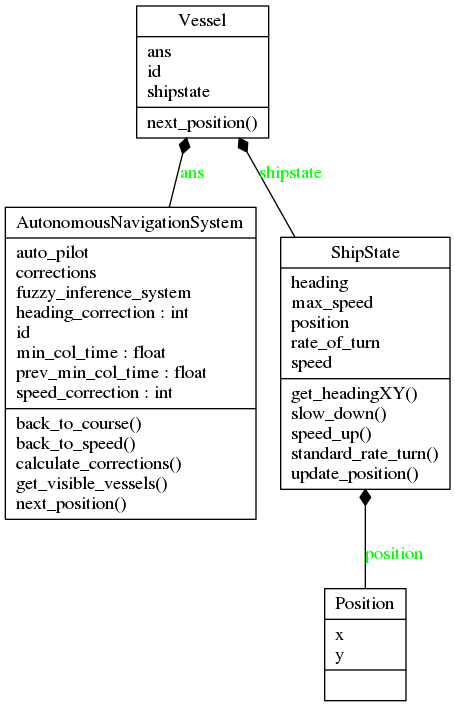
\includegraphics[width=\textwidth,height=0.75\textheight,keepaspectratio]{../src/classes_Pyreverse}
    \caption{Class diagram}
    \label{fig:class_diagram}
\end{figure}
\subsection{Classes}
Each simulation scenario consists of at least one vessel. These vessels are represented by the \textit{Vessel} class. The current state of the vessel is represented by the \textit{ShipState} class which also contains the \textit{Position} class. Furthermore, each vessel need a navigation system, which is represented by the \textit{AutonomousNavigationSystem} class. The classes will be more thoroughly presented in the following subsections.
\subsubsection{Vessel}
\textit{Vessel} is the main class and the class with which the simulation script interacts.
It contains, apart from the previously mentioned \textit{AutonomousNavigationSystem} and \textit{ShipState} an id and a method to calculate it's position in the next time frame.
A new vessel object in created with the following call:
\begin{minted}{python}
Vessel(id, heading, position_x, position_y, speed, max_speed, 
    rate_of_turn, fuzzy_inference_system, auto_pilot)
\end{minted}
This constructor call specifies the ID for the vessel as well as its initial position, speed and heading. Furthermore it defines the vessels maximum speed and rate of turn. The two final parameters specify the fuzzy inference system to use and whether the vessel shall use the navigation system. Setting the final boolean to false creates a rogue vessel that will just keep its initial speed and heading, thereby not complying to the COLREG rules. The \textit{Vessel} class has one just one method, which calculates the vessels position in the next time frame after applying possible corrections to heading ans speed.
\subsubsection{Position}
The position class simply holds the vessels current coordinates in the Cartesian coordinate system used.
\subsubsection{ShipState}
ShipState holds information about the state of the vessel in the current time frame. This includes the vessels current position, heading and speed. The simulation does not distinguish between course and heading since no drift is simulated.
Furthermore, limits such as maximum allowed speed and standard rate of turn is specified in this class. Finally, the class holds methods to change the ships heading by the specified standard rate of turn or speed by 1, for the next time frame.


\subsubsection{AutonomousNavigationSystem}
The AutonomousNavigationSystem class from now on referred to as ANS is what separates an autonomous vessel from an ordinary vessel. The ANS combines the information from the ShipState class with situational awareness information provided by a separate Situational Awareness (SA) module, in order to calculate needed corrections to speed and course.

The SA is in this simulation case represented by a service that holds all information regarding the current scenario. A real system would have a SA module that reads and processes information from different sensors, such as LiDAR, cameras, on board the vessel. Information needed about a target vessel is its heading, speed, and position. These are used to calculate the four different inputs to the FIS system. Listing \ref{listing:rel_bear_calc} shows the method used to calculate the relative bearing fed into the FIS system. Compass bearing is first calculated from the two provided coordinate pairs after which the result is converted into a relative bearing. Relative course is then calculated as the observed vessels heading - the own vessels heading, as shown in listing \ref{listing:rel_course_calc}. Distance can be obtained by using the Pythagorean theorem on the differences between the vessels in the X and Y axis. Finally speed ratio is defined as $\frac{\text{Speed of the observed vessel}}{\text{Speed of the own vessel}}$.
\begin{listing}

    \begin{minted}[linenos, breaklines=true,fontsize=\scriptsize, numberblanklines=false]{python}
rel_course = observed_vessel.shipstate.heading - shipstate.heading
if rel_course < 0:
    rel_course = 360 + rel_course
    \end{minted}
    \caption{Relative course calculation}
    \label{listing:rel_course_calc}
\end{listing}

Furthermore the expected time until collision needs to be calculated for each target vessel to prioritize the recommended corrections. Knowing the distance between the vessels, their relative velocity is needed to calculate the time. Equation \ref{eq:rel_vel_calc} shows the relative velocity calculation, based on the law of Cosines. \textit{V} stands for velocity, $\theta$ for heading, the subscript \textit{m} for own vessel and \textit{t} for target vessel.

\begin{equation}
    V_r=\sqrt{V_m^2 + V_t^2-2  V_mV_tcos(\theta_m-\theta_t)}
    \label{eq:rel_vel_calc}
\end{equation}


% \begin{listing}

%     \begin{minted}[linenos, breaklines=true,fontsize=\scriptsize, numberblanklines=false]{python}
% vm = shipstate.speed
% vt = observed_vessel.shipstate.speed
% cm = math.radians(shipstate.heading)
% ct = math.radians(observed_vessel.shipstate.heading)
% vr = math.sqrt(pow(vm, 2) + pow(vt, 2) - 
%     2 * vm * vt * math.cos(cm - ct))
% distance = helpers.distance(shipstate.position, observed_vessel.shipstate.position)

% time_until_collision = distance / vr
%     \end{minted}
%     \caption{Expected time until collision calculation}
%     \label{listing:colt_time_calc}
% \end{listing}













\subsection{Simulation}
The goal of the implementation is to simulate a real word situation with respect to time, speed, acceleration, and rate of turn, while neglecting  environmental factors such as weather. The simulation is therefore limited to two dimensions in a Cartesian coordinate system, in which the scenario is updated with one second intervals.



\chapter{Scenarios}
